% IEEE Transactions-style rebuttal.
% IEEEtran is included in standard Overleaf TeX Live installations.
\documentclass[journal,10pt]{IEEEtran}

\usepackage{graphicx}
\usepackage{amsmath}
\usepackage{amssymb}
\usepackage{booktabs}
\usepackage{xcolor}
\usepackage{lipsum} % Only used for the placeholder text below.
\usepackage[hidelinks]{hyperref}

% Support for easy cross-referencing
\usepackage[capitalize]{cleveref}
\crefname{section}{Sec.}{Secs.}
\Crefname{section}{Section}{Sections}
\Crefname{table}{Table}{Tables}
\crefname{table}{Tab.}{Tabs.}

\definecolor{responseblue}{RGB}{0,70,160}

\newcommand{\reviewer}[1]{%
  \par\smallskip\noindent
  \textcolor{responseblue}{\textbf{#1\hspace{0.2em}}}%
}

\newcommand{\question}[2]{%
  \par\smallskip\noindent
  \textcolor{responseblue}{\textbf{Q#1: #2}}%
  \par\nobreak\noindent
}
\newcommand{\answer}{%
  \par\smallskip\noindent
  \textbf{Answer: }\ignorespaces
}

% If you wish to avoid re-using figure, table, and equation numbers from
% the main paper, please uncomment the following and change the numbers
% appropriately.
%\setcounter{figure}{2}
%\setcounter{table}{1}
%\setcounter{equation}{2}

% If you wish to avoid re-using reference numbers from the main paper,
% please uncomment the following and change the counter for `enumiv' to
% the number of references you have in the main paper (here, 6).
%\let\oldthebibliography=\thebibliography
%\let\oldendthebibliography=\endthebibliography
%\renewenvironment{thebibliography}[1]{%
%     \oldthebibliography{#1}%
%     \setcounter{enumiv}{6}%
%}{\oldendthebibliography}


% Rebuttal metadata -- update these two fields.
\newcommand{\PaperID}{26-0767}
\newcommand{\PaperTitle}{Simultaneous Contact Selection and Planning for Contact-Rich Manipulation with Cascaded Optimization}

\begin{document}

\title{\LARGE\bfseries Response to Reviewers\\
  \normalfont\normalsize Manuscript ID: \PaperID\\
  \normalfont ``\PaperTitle''}
\maketitle

% BODY TEXT -- enter your response below.
We thank all three reviewers for their constructive comments and for highlighting the strengths of our work, including that SCSP addresses a real limitation of local contact-implicit model predictive control (CIMPC) methods (\textbf{R1}) and a real gap in existing CIMPC methods (\textbf{R2}), the proposed contact selection and ranking strategy is practical and effective (\textbf{R1}, \textbf{R3}), and that the experiments are thorough and extensive (\textbf{R3}) and above average for this literature (\textbf{R2}), with strong results across simulation and real-world hardware experiments without motion capture (\textbf{R1--R3}).


\reviewer{Reviewer 1}

\question{1}{The CSO-as-MIQP claim is under-specified}

Section III-D states that Eq. (32) is formulated as an MIQP, that the inner loop constitutes a QP, and that the overall CSO is an efficient MIQP. This is plausible only under additional assumptions that are not made explicit.

For a fixed sampled contact point, fixed contact geometry, fixed Jacobians, quadratic objective, polyhedral friction constraints, and an explicit active-set or binary-variable encoding of
\begin{equation}
    \hat{\lambda}_{\text{env},i}=\max(A_i\hat{\lambda}_r+b_i,0),
\end{equation}
the problem can be written as a region-wise QP or as an MIQP. However, the paper does not provide the MIQP variables, big-$M$ or indicator constraints, active-set constraints, or the precise quadratic form being solved. The implementation section also states that the CSO inner loop is solved using CasADi with SNOPT, which is an SQP/NLP solver rather than a QP or MIQP solver.

The paper should either present the exact QP/MIQP formulation and solver details, or weaken the claim to finite candidate search with local continuous force optimization under an SCM approximation.

\answer
Thank you for pointing out this inconsistency. We agree that our
previous characterization of CSO as an MIQP, and of its inner problem
as a QP, was imprecise.

In our actual implementation, the sampled contact location is not
encoded as an integer decision variable, and we do not introduce
binary variables, big-$M$ constraints, indicator constraints, or use
a mixed-integer solver. Instead, the discrete contact-location variable
is handled explicitly through the finite candidate set
$\mathcal{I}_{\mathrm{avail}}$. For each candidate contact location,
we solve a continuous optimization problem over the robot contact
forces and then compare the resulting costs across candidates.

Moreover, although the SCM makes the environment contact force an
explicit piecewise-linear function of the robot contact force,
\begin{equation}
    \hat{\lambda}_{\mathrm{env}}
    = \max(A\hat{\lambda}_r+b,0),
\end{equation}
this mapping is picewise-linear but nonsmooth at active-set transitions. Therefore, the
resulting inner problem is not, in general, a QP. In the implementation,
it is solved as a low-dimensional piecewise-smooth constrained
nonlinear optimization problem using S.

We have revised the manuscript accordingly. Specifically, we no longer
refer to CSO as an MIQP or its inner optimization as a QP. Instead, we
describe CSO as a paralleled optimization consisting of a
finite search over sampled contact locations and lightweight continuous force
optimization under the SCM approximation. We have also corrected the
statement regarding the regularity of Eq.~(28): the mapping itself is
piecewise linear and Lipschitz continuous, but its Jacobian is only
piecewise defined and may be discontinuous at active-set boundaries.
These revisions make the mathematical description consistent with the
actual solver used in our implementation.
\question{2}{The SCM assumptions and error bound are too weak}

The surrogate contact model relies on fixed object-environment contact sets and decoupled multi-contact dynamics. These are strong assumptions, especially during flipping, tipping, rolling, or simultaneous multi-contact interaction. Lemma 3 only gives a boundedness argument; it does not establish accuracy or useful dependence on contact geometry, active-set changes, force magnitude, or the off-diagonal blocks of the Delassus matrix.

The paper should state the regularity assumptions required for Lipschitz continuity of the LCP solution and provide empirical SCM error validation against a higher-fidelity contact solver.
\answer
Thank you for this important comment. We agree that SCM relies on strong assumptions and should include a more thorough analysis of modeling errors. Our motivation is that high-fidelity contact dynamics and complete contact detection are both nonsmooth and computationally expensive for optimization. Moreover, high-fidelity contact dynamics are highly geometry-dependent and involve nonsmooth contact transitions, which can introduce numerical instability during optimization. Therefore, the role of SCM is only to predict the correct object motion trend rather than provide high-fidelity contact simulation. In practical deployment, the influence of SCM approximation errors on SCSP is further alleviated by the high-frequency receding-horizon updates of the framework.

We have
strengthened both the theoretical analysis and the empirical
validation as below:

\textbf{1) Theoretical Analysis:}
We first explicitly state the regularity condition of the contact LCP.
Recall that
\[
W_{\rm env}
=
\widetilde J_{\rm env}M_o^{-1}
\widetilde J_{\rm env}^{\top}+R,
\]
where $R\succeq r_{\min}I$, $r_{\min}>0$, is a regularization term
introduced for numerical stability. Therefore,
$W_{\rm env}\succeq \mu I$ and the corresponding contact optimization
problem is strongly convex with a unique solution.

For two regularized contact problems $(W_1,g_1)$ and $(W_2,g_2)$ with
solutions $\lambda_1$ and $\lambda_2$, the associated variational
inequalities give
\[
\|\lambda_1-\lambda_2\|_2
\leq
\frac{1}{\mu}
\left(
\|g_1-g_2\|_2
+
\|W_1-W_2\|_2\|\lambda_2\|_2
\right).
\]
This establishes the local Lipschitz sensitivity of the regularized
LCP solution with respect to perturbations of contact geometry and
contact dynamics.

In particular, contact geometry affects the LCP coefficients through
$\widetilde J_{\rm env}$, which is constructed from contact locations
and local contact frames obtained by the contact detector. Therefore,
for a fixed contact topology, locally bounded perturbations of contact
geometry induce bounded perturbations of $W_{\rm env}$ and the LCP
solution.

We further clarify that the geometric contact set and the LCP active set
are different concepts. Assumption~1 fixes the candidate geometric
contacts within one SCM rollout, but does not require all contacts to
remain active. Existing contacts can become inactive by taking zero
contact force. Since the above variational inequality does not assume
identical active sets between two solutions, activation/deactivation of
retained contacts is covered by the sensitivity analysis.

Based on this sensitivity result, we analyze the approximation error
introduced by SCM.
Let $D$ denote the diagonal Delassus approximation adopted by SCM.
Setting $W_1=W_{\rm env}$, $W_2=D$, and $g_1=g_2$ gives

\begin{equation}
\|\lambda_{\rm env}-\widehat{\lambda}_{\rm env}\|_2
\leq
\frac{\|W_{\rm env}-D\|_2}{\mu}
\|\widehat{\lambda}_{\rm env}\|_2 .
\end{equation}

Accordingly, the one-step state prediction error is bounded by

\begin{equation}
\|x_{k+1}-\widehat{x}_{k+1}\|_2
\leq
\underbrace{
\frac{\|M_o^{-1}\widetilde{J}_{\rm env}^{\top}\|_2}{\mu}
\|W_{\rm env}-D\|_2
\|\widehat{\lambda}_{\rm env}\|_2
}_{E_{\rm SCM}} .
\end{equation}

This bound provides a direct physical interpretation of the SCM
approximation error. Specifically, $\widetilde{J}_{\rm env}$ reflects
the influence of contact geometry, $\|W_{\rm env}-D\|_2$ characterizes
the neglected Delassus coupling between contacts, including the
off-diagonal blocks, and $\|\widehat{\lambda}_{\rm env}\|_2$ represents
the influence of contact-force magnitude.

\textbf{2) Active-set changes:}
The above bound assumes that the geometric contact set considered by SCM
remains unchanged within one rollout. In practice, active-set changes
can be categorized into contact removal and contact creation.

For contact removal, SCM retains the corresponding geometric contact
constraint but allows the contact force to become zero. Therefore, the
detached contact does not introduce additional wrench, and the resulting
prediction error remains bounded by the above sensitivity analysis.

In contrast, newly created contacts are absent from the current SCM
rollout. Their contact locations, Jacobians, and forces are unknown
during optimization, and therefore their influence cannot be bounded by
the above sensitivity analysis without additional assumptions. The total
prediction error can therefore be conceptually decomposed as

\begin{equation}
E_{\rm total}
\leq
E_{\rm SCM}+E_{\rm new},
\end{equation}

where $E_{\rm SCM}$ corresponds to the approximation error under the
current contact topology and $E_{\rm new}$ represents the uncertainty
introduced by newly generated contacts.

In practical SCSP execution, the contact state is updated at every
receding-horizon optimization step. Consequently, newly generated
contacts are incorporated into subsequent SCM updates, preventing
$E_{\rm new}$ from accumulating over long horizons. Therefore, SCM is
used as a computationally efficient contact-trend predictor rather than
a high-fidelity long-horizon contact simulator.

\textbf{3) Empirical validation.}
Finally, we add an empirical comparison between SCM and a
higher-fidelity contact solver under representative contact
configurations, including contact transitions and multi-contact cases.
We report the one-step object-motion prediction error and motion
direction/ranking consistency, which directly evaluate whether SCM
preserves the motion tendency required by CSO despite its simplified
contact dynamics.

\question{3}{The ranking strategy appears internally inconsistent}

The paper defines
\begin{equation}
    \rho=\frac{\ell_{\text{near}}-\hat{\ell}_{\text{min}}}{\max(\hat{\ell}_{\text{max}}-\hat{\ell}_{\text{min}},\epsilon)}.
\end{equation}
With this definition, smaller $\rho$ means that $p_{\text{near}}$ is closer to the best candidate, and larger $\rho$ means it is worse. However, Eq. (39) sets $\kappa_t=\mathbf{1}(\rho_t>\bar{\rho})$ and states that $\kappa_t=1$ means $p_{\text{near}}$ is sufficiently good. This reverses the intended meaning. Eq. (40) is also difficult to reconcile with Algorithm 2 and the described lifting/placing phases.

This section should be rewritten as a clear finite-state or hysteresis rule. As written, the trigger logic is not mathematically consistent.

\answer
Thank you for pointing out this inconsistency. We agree that the original definition of the ranking score was unclear and could lead to a reversed interpretation. In the revised manuscript, $\rho_t$ is explicitly defined as the normalized ranking score of $p_{\mathrm{near}}$ based on its cost reduction $\Delta \ell_t^{\mathrm{near}}$ and the range of cost reductions $[\Delta \ell_t^{\mathrm{min}},\Delta \ell_t^{\mathrm{max}}]$ among all candidate contact locations:
\begin{equation}\label{equ:ranking1}
\rho_t=
\Pi_{[0,1]}\!\left(
\frac{
\Delta\ell_t^{\mathrm{near}}
-\Delta\ell_t^{\mathrm{min}}
}{\max(
\Delta\ell_t^{\mathrm{max}}
-\Delta\ell_t^{\mathrm{min}}, \epsilon)
}
\right)
\end{equation}
It represents the relative ranking of the improvement achieved by $p_{\mathrm{near}}$ compared with other candidates. Therefore, a smaller $\rho_t$ indicates that $p_{\mathrm{near}}$ provides less improvement and has a worse ranking, while a larger $\rho_t$ indicates that $p_{\mathrm{near}}$ is more competitive.

We further clarify that the previous formulation using the absolute cost $\ell$ and the revised formulation using the cost reduction $\Delta\ell$ are equivalent under min-max normalization, except for the ordering convention. Specifically, since the cost reduction is defined as $\Delta \ell_t^i
=\ell(\boldsymbol{x}_t)-\ell(\hat{\boldsymbol{x}}_t^+)$, we can obtain that
\begin{equation}
\rho_t
=
\Pi_{[0,1]}\!\left(\frac{
\ell(\hat{\boldsymbol{x}}_{t}^{+,\mathrm{min}})
-
\ell(\hat{\boldsymbol{x}}_{t}^{+,\mathrm{near}})
}{
\max(
\ell(\hat{\boldsymbol{x}}_{t}^{+,\mathrm{min}})
-
\ell(\hat{\boldsymbol{x}}_{t}^{+,\mathrm{max}}),
\epsilon)
}\right). \label{equ:correct_derivation}
\end{equation}
The above derivation shows that the previous formulation using the absolute cost $\ell$ was equivalent in principle but introduced ambiguity due to the reversed ordering convention. To avoid this confusion, we have rewritten the Ranking Strategy subsection in Section IV-B and reformulated $\rho_t$ directly based on the cost reduction $\Delta\ell$. This revision improves the clarity and consistency of the ranking interpretation while keeping the underlying strategy unchanged.

\question{4}{The CPO potential costs appear incorrectly specified}

The lifting cost uses
\begin{equation}
    \ell_{\text{obs}}=\log(\lVert p_{\text{ee}}-p_o\rVert^2+\epsilon),
\end{equation}
inside a distance threshold and minimizes it. This is not a repulsive potential unless the weight is negative, which is not stated. The placing cost says that $\ell_{\text{con}}$ attracts the end-effector to the reference contact point $p_{\text{ref}}$, but the formula uses $p_o$ instead of $p_{\text{ref}}$:
\begin{equation}
    \ell_{\text{con}}=\log(\lVert p_{\text{ee}}-p_o\rVert^2+\epsilon).
\end{equation}
This should be corrected or explained. A natural formulation would explicitly include a term such as $\lVert p_{\text{ee}}-p_{\text{ref}}\rVert^2$.

\answer
Thank you for identifying these inconsistencies. We have revised Section IV-C (highlighted in red). Specifically, the sign of the object repulsive potential $\ell_{\mathrm{obs}}$ has been corrected to ensure a repulsive behavior, and the contact attraction term $\ell_{\mathrm{con}}$ has been modified to explicitly attract the end-effector toward the reference contact point $\boldsymbol{p}_{\mathrm{ref}}$.

\question{5}{The result analysis does not isolate the proposed contributions}

The experiments mainly show that the full SCSP system outperforms several baselines in aggregate success rate. They do not sufficiently explain which proposed mechanism causes which improvement. The causal link between the stated contributions and the results is therefore incomplete.

In particular, the paper should report evidence for each component:
\begin{itemize}
    \item CSO: quality of selected contact priors, contact-location maps, correlation between CSO cost and execution success, and comparison against random, nearest, heuristic, and multi-start contact selection.
    \item SCM: prediction error against a higher-fidelity contact solver, separated by contact count, contact mode, object geometry, and flipping/rotation phase.
    \item Ranking strategy: switch frequency, time spent tracking $\hat{p}_r^*$ versus $p_{\text{near}}$, failure cases caused by switching, and sensitivity to $\bar{\rho},T_1,T_2,T_3$.
    \item CPO objective: ablation of lift, place, object-center attraction, and $p_{\text{ref}}$ tracking terms.
    \item Robustness: failure categories separating perception error, contact estimation error, slippage, control saturation, and poor prior selection.
\end{itemize}
Without these analyses, claims about robustness, diversity, and the specific benefit of each module remain qualitative.

\question{6}{Baseline coverage and comparison protocols need strengthening}

The Sampling comparison is not fully controlled because the paper replaces the original contact model with $f_{cf}$. This may create a new baseline rather than a direct implementation of the cited method. The DyWA comparison also needs careful framing: DyWA is described in Table I as lacking generalization, although its stated purpose is generalizable nonprehensile manipulation. The paper should define exactly what ``generalization'' means.

The baseline set is also incomplete relative to the scope of the claims. The following comparisons or discussions are particularly relevant:
\begin{itemize}
    \item STOCS / STOCS-3D: this is the closest prior work in spirit, since it directly addresses simultaneous trajectory optimization and contact selection with high-fidelity geometry. Even if it is not real-time, it should be used as an offline planning-quality reference or excluded with a clear justification.
    \item ContactSDF: this should be discussed for the paper's multi-contact, differentiable contact-model, and dexterous-manipulation claims. If a direct comparison is not feasible, the paper should explain the domain difference and narrow the multi-contact claims.
    \item Generic sampling-based optimizers: the paper should compare against MPPI, CEM, CMA-ES, or random shooting under the same dynamics model, cost, action parameterization, horizon, and wall-clock budget. Otherwise it is unclear whether SCSP's improvement comes from its contact-selection structure or simply from spending computation on sampled contact/control candidates.
\end{itemize}
A useful protocol would include both contact-location sampling baselines, e.g., CEM/CMA-ES over $p_r$ and $\lambda_r$, and control-sequence sampling baselines, e.g., MPPI/CMA-ES over end-effector waypoints or joint commands without CSO. These should be run with the same model and compute budget as SCSP.

\begin{figure*}[htbp]
    \centering
    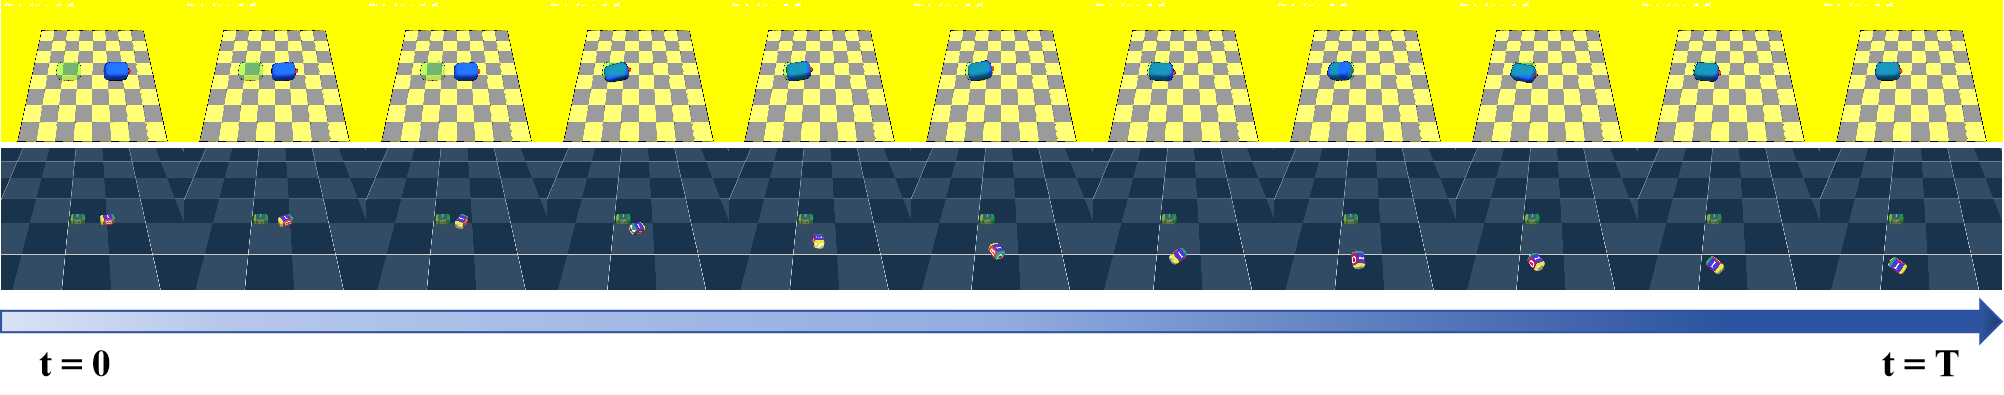
\includegraphics[width=\linewidth]{figures/stocs_track.png}
    \caption{
    Comparison between the trajectory planned by STOCS-3D (top) and its execution through contact-force tracking in MuJoCo (bottom). Although STOCS-3D produces a reasonable planned trajectory, the objec gradually deviates from the predicted trajectory during execution due to the mismatch between the quasi-dynamic planning model and the full contact dynamics in MuJoCo.
    }
    \label{fig:stocs_tracking}
\end{figure*}

\textbf{Answer:}
We thank the reviewer for the valuable suggestions. We have revised the baseline implementation and clarified the comparison protocols in the revised manuscript.

For the Sampling baseline, the original comparison replaced its contact model with $f_{cf}$ to isolate the influence of the upper-level contact guidance. However, we agree that this modification may change the original baseline. Therefore, we have re-implemented Sampling following the official implementation provided by the original paper and updated the success rates of all experiments accordingly.

For DyWA, we clarify that the ``generalization'' in the original Table I was ambiguous. DyWA focuses on cross-object generalization, whereas our discussion refers to multi-task and cross-embodiment generalization. We have revised the description in Table I to ``multi-task generalization'' to avoid confusion.


STOCS-3D formulates contact-rich manipulation as an MPCC and uses D-SDF to preserve multi-contact coupling with higher contact fidelity than SCM. However, it performs offline optimization with a fixed robot--object contact attachment and does not explicitly search for optimal contact locations. We therefore execute the wrench trajectory planned by STOCS-3D using our CPO framework at the same contact location. Due to execution errors under full contact dynamics, STOCS-3D achieves only 3\% success on the first task and 0\% on the remaining six tasks, compared with 79--100\% for SCSP. This highlights the importance of closed-loop replanning and active contact selection.

ContactSDF provides a differentiable multi-contact model but does not explicitly perform global search over feasible object surface contacts. Instead, contacts are generated through attraction-based optimization. In contrast, SCSP treats contact location as an explicit decision variable through CSO. ContactSDF achieves 0--12\% success across the seven tasks, while SCSP achieves 79--100\%, demonstrating the benefit of explicit contact selection.

\question{7}{Multi-contact and generalization claims are overstated}

The notation allows multiple robot contact points, and the SCM includes multiple environment contacts. However, the main nonprehensile manipulation experiments use point-contact end-effectors, and the SCM explicitly neglects coupling between environment contacts. The later soccer, grasping, and long-horizon experiments are useful case studies, but they do not establish a general simultaneous multi-contact planning capability.

The claim that SCSP can be easily extended to multi-contact tasks should be weakened. The paper should discuss scalability with respect to the number of robot contacts, since selecting $n_r$ contacts from $n_s$ candidates can scale combinatorially, e.g., $\binom{n_s}{n_r}$ in the unordered case.

\answer 
Thank you for pointing out this important limitation. We agree that extending SCSP to general multi-contact tasks faces scalability challenges. In Section VI-A(3), we demonstrate that SCSP can autonomously select finger contacts and generate force-closure grasps without manually specifying contact locations or the number of fingers. By leveraging GWB-based methods to reduce the CSO search space, this result demonstrates the potential of SCSP for extending contact selection and planning to multi-contact manipulation. 

However, we acknowledge that more complex multi-contact tasks involve not only combinatorial growth but also strong geometric coupling among contact locations, which remain challenging for the current SCSP framework. The demonstrated precision grasping case involves a limited number of contacts with relatively weak coupling among fingers, while more complex tasks such as power grasping remain challenging for autonomous planning. We have therefore weakened our claims in the revised manuscript, stating that SCSP provides a potential framework for multi-contact manipulation rather than a general solution. This limitation and the scalability of multi-contact planning are also discussed as future work in Section VII.multi-contact planning are also discussed as future work in Section VII.


\question{8}{Hardware evidence is encouraging but statistically limited}

The real-world experiments use only five trials per object/surface condition. This is too small to support strong robustness claims. The paper should either increase the number of trials or report confidence intervals and failure categories. It should also report how often failures come from perception, contact estimation, slippage, control saturation, or poor contact prior selection.

\answer 
Thank you for pointing out this limitation. We have increased the number of real-world trials from 5 to 20 and report the failure categories in the revised Table IV, including slippage (reflecting the effectiveness of contact switching strategies), exceeding the operational range (reflecting the recovery capability of different methods), and improper contact prior selection (reflecting the quality of the selected contact locations).

The effects of perception and contact estimation errors are more difficult to quantitatively isolate. Their influence on SCSP and Sampling is reflected through inaccurate contact location generation and model mismatch in contact planning, while DyWA, as an end-to-end method with partial point cloud inputs, is even less interpretable in this regard. Therefore, we do not separately evaluate these factors. In our experiments, perception failures are mainly observed in severe occlusion cases causing object pose estimation failures, which rarely occur in the tested scenarios.
\question{9}{Technical Corrections}

\begin{itemize}
    \item The friction constraints in Eq. (32) should include both signs of each tangential component, e.g.,
    \begin{equation}
        |\hat{\lambda}_{r,i}^{t1}|\leq\mu_i\hat{\lambda}_{r,i}^{n},
        \qquad
        |\hat{\lambda}_{r,i}^{t2}|\leq\mu_i\hat{\lambda}_{r,i}^{n}.
    \end{equation}
    \item SCM is called ``smooth,'' but the max operator is piecewise linear and nonsmooth at the switching surface.
    \item Eq. (35) should be rechecked for units and consistency between force and impulse notation.
    \item The text refers to the optimal contact location as $\hat{\lambda}_r^*$ in one place; this should be $\hat{p}_r^*$.
    \item The quaternion error in Table II is labeled as radians, but the reported metric appears to be $1-(\psi^T\psi_g)^2$, not an angular error in radians.
    \item Lemma 4 is not a proof of non-conflicting objectives. It should be removed, weakened, or replaced with a precise first-order condition.
\end{itemize}

\answer We thank the reviewer for the careful checking of the technical details. We have revised Eq. (32) and Eq. (35) to ensure the correctness of the friction constraints and the consistency of force/impulse notation. We have also corrected the notation error after Eq.(32) by replacing $\hat{\boldsymbol{\lambda}}_r^*$ with $\hat{\boldsymbol{p}}_r^*$, removed the incorrect radian unit annotation in Table II, and clarified that the quaternion error metric is a dimensionless quantity.

For the terminology of SCM, we agree that the max operator introduces piecewise linearity and nonsmoothness. We have revised the description from ``\textit{smooth and computationally efficient formulation}'' to ``\textit{computationally efficient formulation}''.

Finally, we have weakened the statement of Lemma 4. Instead of claiming a formal proof of non-conflicting objectives, it is now presented as an intuitive discussion of the relationship between the objectives.

\reviewer{Reviewer 3}

\question{1}{Contradictory ranking-strategy definitions}

The ranking strategy contains contradictory definitions as printed. In
(38), $\rho$ is normalized so $\rho \sim 0$ means $p_{\mathrm{near}}$ is close to the best
candidate, and (39) sets $\kappa = 1$ when $\rho > 0.75$, i.e., $\kappa = 1$
marks $p_{\mathrm{near}}$ as a poor candidate. Under this reading, (40), Fig. 6, and
Algorithm 2 are mutually consistent ($\mathrm{infeasible} \rightarrow \gamma = 0 \rightarrow$ lift
toward the CSO optimum). But the sentence directly below (39) states
the opposite, that $\kappa = 1$ indicates $p_{\mathrm{near}}$ is "sufficiently good,"
and the sentence introducing the trigger defines "a trigger variable
$\gamma$" and then writes the formula for $\kappa$. In addition, both
branches of (40) gate on the same counter $t_{(\kappa=1)}$, defined after
Algorithm 2 as the total timesteps satisfying $\kappa = 1$; I suspect
the first branch should use $t_{(\kappa=0)}$, and it is not stated whether
the counters are cumulative or consecutive, or when they reset. As written,
the placing branch triggers only after $T_1$ accumulated infeasible steps,
which does not match the described behavior. Please correct the prose
and (40) from the implementation and define the counter semantics; at
present the switching logic cannot be implemented unambiguously.

\answer Thank you for the careful observation. We agree that the original formulation contained inconsistencies between the definition of $\rho$, the interpretation of $\kappa$, and the switching logic. The ambiguity mainly originated from a derivation error when simplifying the original formulation.

In the revised manuscript, we have rewritten Section IV-B and reformulated $\rho_t$ with a clearer definition. Specifically, for each candidate contact location $p_i \in \mathcal{I}_{\mathrm{avail}}$, the optimal contact force $\boldsymbol{\lambda}_i^*$ is solved to obtain the corresponding optimal cost reduction $\Delta \ell_t^i = \ell(\boldsymbol{x}_t)-\ell(\hat{\boldsymbol{x}}_t^+)$. The ranking score $\rho_t$ then measures the relative ranking of the cost reduction obtained by $p_{\text{near}}$ among all candidate contact locations. Therefore, $\rho_t$ is reformulated as follows:

\begin{equation}
\rho_t=
\Pi_{[0,1]}\!\left(
\frac{
\Delta\ell_t^{\mathrm{near}}
-\Delta\ell_t^{\mathrm{min}}
}{
\max(
\Delta\ell_t^{\mathrm{max}}
-\Delta\ell_t^{\mathrm{min}},\epsilon)
}
\right).
\end{equation}
With this definition, a larger $\rho_t$ indicates that $p_{\mathrm{near}}$ provides greater improvement and has a better ranking. Accordingly, $\kappa_t=\boldsymbol{1}(\rho_t>\bar{\rho})$ consistently indicates whether $p_{\text{near}}$ is sufficiently good. The previous derivation error was introduced during a further simplification of the formulation, as shown in \eqref{equ:correct_derivation}.

We also corrected the switching rule in (40) and clarified the counter semantics. The counters $t_{(\kappa=1)}$ and $t_{(\kappa=0)}$ now represent the consecutive timesteps satisfying $\kappa=1$ and $\kappa=0$, respectively, and are reset when the corresponding condition is violated. These revisions remove the ambiguity in the switching logic while keeping the original ranking strategy unchanged.

\question{2}{Optimization claims}

CSO performs a global search over the sampled candi-
date set, not over the continuous surface, so ``globally opti-
mal” (Fig. 2 caption) and especially ”asymptotically optimal”
(after (32), where the symbol should also be $\hat{p}^{}_{r}$, not
$\hat{\lambda}^{}_{r}$) are overclaims; please reword or prove. The
paper calls the problem an MIQP with sub-millisecond QP
subproblems, but the implementation uses SNOPT, an SQP
solver for NLPs, and with the quaternion cost the subproblem
is not a QP. Algorithm 1 is titled ”Sampling and Exchange
Method” and Table V lists an ”Exchange cost time,” but no
exchange step is defined anywhere. Since $70 \times 0.23$ ms is
about the reported 16 ms CSO time, I assume the candidates
are simply enumerated; if so, just say so.

\answer Thank you for pointing out these inconsistencies. We agree that our previous descriptions of CSO as an MIQP and its inner optimization as a QP were imprecise. Since the discrete contact variable is not formulated with binary variables, big-$M$ constraints, or a mixed-integer solver, CSO is no longer described as an MIQP. Moreover, due to the piecewise-linear but nonsmooth contact force mapping
\begin{equation}
    \hat{\lambda}_{\mathrm{env}}=\max(A\hat{\lambda}_r+b,0),
\end{equation}
the inner problem is not generally a QP. It is implemented as a low-dimensional constrained nonlinear optimization problem. We have revised the corresponding descriptions accordingly.

We also agree that the terms ``globally optimal'' and ``asymptotically optimal'' were overstated. Since the optimization is performed only over a sampled candidate set rather than the continuous contact surface, we have weakened these statements to ``optimal among the sampled candidates'' and removed the asymptotic optimality claim. The notation in Eq.~(32) has also been corrected from $\hat{\boldsymbol{\lambda}}_r^*$ to $\hat{\boldsymbol{p}}_r^*$.

Regarding the ``exchange'' operation, it refers to reading the current environment contact state and constructing the active candidate set for CSO. We agree that this operation is not a major optimization component. It was included only for completeness in the reporting of the overall CSO wall-clock time. and the previous terminology was misleading. We have clarified its definition in Algorithm 1 and Table V, and removed the ambiguity in the computational cost description.

\question{3}{Text vs. tables}
Sec. V-C states SCSP achieved a 100\% success rate in
on-ground rotation, but Table IV shows 19/20 (Duck, rough surface:
4/5). The open-loop numbers for the long-horizon tasks are missing from
Table VI although the text calls the rates "comparable." Tables IV and
VI say "(\%)" but list raw counts. "Significantly outperforms" is not
accurate for multi-finger grasping (16/20 vs 15/20). Please reconcile
all of these. I would also suggest confidence intervals: with n = 200
they are trivial to add, and with n = 5 per hardware cell the current
wording is stronger than the data supports.

\answer Thank you for the suggestions. We agree that the original description contained several inconsistencies. In the previous experiments, Duck failed once in the on-ground rotation task. Following Reviewer 1's suggestion, we increased the number of trials and repeated the experiments, achieving a success rate of 79/80. Therefore, we have revised ``\textit{achieved a 100\% success rate}'' to ``\textit{achieved a nearly 100\% success rate}''. 

The missing open-loop results for the long-horizon tasks were caused by a LaTeX compilation issue, and we have added them in the revised Table VI. We have also changed ``\textit{significantly outperforms}'' to ``\textit{outperforms}'' for multi-finger grasping to avoid overstating the improvement. 

Furthermore, the previous number of real-world trials was insufficient for confidence interval estimation. After increasing the trials to 20 for each hardware condition, we have added confidence intervals to both Table IV and Table VI.


\question{4}{Reproducibility}
The friction-cone constraints in (32) have no lower\
bounds on the tangential components as printed (and $n_t$ vs $n_d$ is\
inconsistent with (9)); please print the exact constraints used. Values\
for $w_{\text{att}}$, $w_{obs}$, $w_{\text{con}}$, $w_o$ (is this the same as $w_{\text{obj}}$?), $\sigma$, the 
lift offset $d$, and solver settings are missing. Please also mark the\
4.82 s sampling in Table V as offline so the\
real-time claim is unambiguous.

\answer Thank you for pointing out these issues. We have corrected the friction-cone constraints in Eq. (32) by explicitly adding the lower bounds on the tangential components $|\hat{\lambda}_{r,i}^{t1}| \leq \mu_i \hat{\lambda}_{r,i}^{n}, \quad
|\hat{\lambda}_{r,i}^{t2}| \leq \mu_i \hat{\lambda}_{r,i}^{n}$.

We have also corrected the notation inconsistency between $n_t$ and $n_d$. The values of $w_{\text{att}}$, $w_{\text{obs}}$, $w_{\text{con}}$, $w_o$ (renamed consistently with $w_{\text{obj}}$), $\sigma$, the lift offset $d$, and solver settings have been added in the revised experimental section. In addition, the 4.82 s sampling time in Table V has been explicitly marked as ``\textit{Offline sampling cost time}" to avoid ambiguity regarding the real-time performance claim.

\question{5}{Minor comments}
In (33), $\alpha$ is introduced as a weighting coefficient but never used.
$\tilde{Q}$ appears in (8) and (11) but only $Q$ is defined in (4).
In (47), the terminal term is $w_{\text{cso}}\ell_{\text{cso}}$ while the text says $V_f$ as
in (7); the same equation mixes $t$ and $k$ as time indices. In (13) and
(32) the objective carries a free index $k$; presumably $x_T$ is meant.
(18) is undefined when $n_i$ is parallel to the reference axis $a$; please
state the fallback.
Please state the orientation tolerance in (51) in degrees (about $26$
deg) and the distribution behind ``mass randomly scaled within a factor
of 10."
\answer Thank you for pointing out these issues. The $\tilde{\boldsymbol{Q}}$ in (8) and (11) is a notation error and should be $\boldsymbol{Q}$ as defined in (4). We have corrected this inconsistency in the revised manuscript.

For the terminal cost in (47), we clarify that the objective should be defined based on the object trajectory. The previous formulation using $\ell_{\mathrm{cso}}$ was unclear. Specifically, $\ell_{\mathrm{cso}}$ in Eq. (34) is defined as:
\begin{equation}
\ell_{\mathrm{cso}} =
\begin{cases}
\ell_{\mathrm{stab}}, & \text{if } \boldsymbol{x}_o \notin \mathcal{X}_g,\\
\ell_{\mathrm{pose}}, & \text{otherwise}.
\end{cases}
\end{equation}
This formulation does not introduce a new objective, but instead changes the target pose from the final goal pose to an intermediate stable pose when necessary. For example, in flipping tasks, first reaching a stable pose close to the goal pose can improve manipulation success. For long-horizon tasks such as opening a microwave door, the target poses are selected along the geometrically constrained trajectory of the door axis.

To avoid ambiguity, we have revised the description in Section III-D(3). Instead of separately defining $\ell_{\mathrm{cso}}$, $\ell_{\mathrm{pose}}$, and $\ell_{\mathrm{stab}}$, we now use a unified objective $\ell$ with different target states during different planning stages. We have also clarified the stable pose preprocessing procedure in the experiment section.

We have unified the time index in Eq. (47) to $k$, representing the discrete timestep. The free index issue in the objectives of (13) and (32) has also been corrected. We have added a fallback strategy for the local frame construction in Eq.(18). When the reference axis $a$ is nearly parallel to the normal vector $n_i$, another coordinate axis is selected as the reference axis to avoid singularity in the projection operation. The threshold in Eq. (51) was a typographical error. The actual value used in the experiments is $1-(\boldsymbol{\psi}_{\mathrm{goal}}^\top\boldsymbol{\psi}_o)^2\leq 0.015$,
instead of $0.05$. We have corrected Eq. (51) and added the corresponding orientation tolerance and mass distribution details.

\reviewer{Reviewer 5}

\question{1}{Quality}

- The authors cover a large span of CI-MPC works from recent literature
and appropriately denote inspiration for the proposed surrogate contact
model.

- The experimentation is thorough and extensive, each validating the
overall efficacy of SCSP across a broad range of tasks.

- The ranking strategy of contact locations, optimized by contact
selection optimization (CSO) and sliding window switching strategy as
described in Alg. 2, and the various attractive and repulsive
potentials, described in Eqns. 41-46, are fairly engineered and require
significant heuristic tuning, as briefly described at the bottom of
page 11. 

- Yet, this ranking strategy is the single most important component of
SCSP, smoothing out the volatility of contact selection with some
heuristics and yielding superior performance compared to the baseline
methods. Since the ranking strategy is such an integral component of
SCSP, its ablation and contribution characterization should be
elaborated on a good deal more. I am curious how often contact
switching, as defined in Eq. (37)-(40) with the grid-swept parameters, is
actually triggered. Is there a measure of how helpful it is? 

- The authors duly note that the greatly simplified surrogate contact
model (SCM) employed for fast CSO limits optimization to point contacts
and prevents sequential state prediction due to poor simulation
fidelity of complex contact/geometry and deformable objects. This is a
large limitation, but broadly endemic to CI-MPC. 

- Contribution four claims manipulation ``using only vision perception,
without the assistance of markers or motion capture systems." I think
caveating with the one-time manual MuJoCo calibration is necessary
here.

\answer
Thank you for recognizing the importance of the ranking strategy and
providing valuable suggestions. We have made the following revisions
accordingly.

\textbf{1) Contribution of ranking strategy:}
The ranking strategy serves as an important bridge between CSO and CPO.
When the contact guidance generated by CSO changes, the ranking strategy
determines whether to maintain the current contact or switch to the
guided contact. Existing CIMPC methods typically rely on attractive
costs to establish robot-object contact. Once contact is established, it
is difficult to actively adjust the contact location, even if the
current contact cannot generate forces within the friction cone that
effectively reduce the object pose error. Therefore, contact switching
can significantly improve task success rate and execution efficiency.

Regarding the actual triggering frequency of the ranking strategy, we agree that this analysis was missing in the original manuscript. Another reviewer also pointed out that the contribution of the ranking strategy was not sufficiently quantified. In the revised manuscript, we have
added the statistics of contact switching events triggered by the ranking strategy (mean $\pm$ standard deviation) and provided a more detailed metric to characterize its contribution. 

Given the ranking strategy triggered state $s_t$, we evaluate three
strategies: (1) the proposed ranking strategy, (2) strictly following
the CSO-generated contact guidance $\hat{\boldsymbol p}_r^*$, and (3)
always selecting the nearest contact $p_{\rm near}$ (similar to CIMPC
methods). Inspired by reinforcement learning evaluation, we perform
counterfactual rollouts from the same initial state and define a
time-discounted terminal reward:
\begin{equation}
J^b
=
\eta\gamma^{T_s^b}\mathbb{I}(\text{success})
\end{equation}
where $b\in\{\text{RS},\text{optimal},\text{near}\}$ denotes the corresponding strategy,
$T_s^b$ is the timestep when the task is completed and $\gamma=0.9$ is the
discount factor. This design evaluates the final task
outcome while considering the convergence efficiency, without assuming
monotonic pose error reduction during contact-rich manipulation.

To quantify the contribution of the ranking strategy, we compute its
relative advantages over the two alternative strategies separately:

\begin{equation}
A_{\text{RS}-b}
=
\frac{
J^{\text{RS}}-J^{b}
}
{
|J^{b}|+\epsilon
},
\quad
b\in\{\text{optimal},\text{near}\}.
\end{equation}
where $b$ denotes the baseline strategy, including strictly following the CSO-generated contact guidance ($b=\text{CSO}$) and always selecting the nearest contact ($b=\text{near}$). We report the average advantages and the ratio of states with positive
advantages, together with the contact switching frequency, to quantify
how frequently the ranking strategy improves execution compared with
directly following the CSO prior or using only the nearest contact.

\textbf{2)Poor simulation fidelity:} Similar to most CIMPC methods, SCM introduces modeling errors due to contact model simplification, and the point-contact assumption further limits its applicability to deformable objects. However, our experiments show that SCSP maintains robust performance under perturbed physical properties in simulation and without system identification in real-world
experiments. This demonstrates that SCSP tolerates single-step simulation errors, which is further supported by our additional analysis experiments. With high-frequency replanning, such simulation errors do not significantly
affect the contact selection and planning decisions of SCSP. 

SCSP has limitations in highly dynamic tasks and deformable object manipulation. Further extending SCSP may require more expressive simulators, such as neural simulators or world models.

\textbf{3)Clarification of contribution:} 
Although our object pose estimation does not rely on motion capture,
we acknowledge that a one-time coarse calibration was performed for contact
detection to prevent significant contact estimation errors. We have clarified
this detail in the revised contribution statement.
\question{2}{Clarity}

- The bullet points in the ``main contributions" paragraph are mostly
rehashed from the preceding paragraph beginning with ``In this work, ..."
Only one of these large text blocks is necessary. 

- Broadly, Section I uses adjective-dense and redundant phrasing, and
it should get a revision for clarity and concision.

- pg. 6 Sec. III.B: how are semantically unsuitable regions for
manipulation determined? The other heuristics for valid region
selection are similarly underexplained.

- Fig. 9b1-4 legend items and axes are hard to read. To accommodate
this, the Fig. 9a1-4 panels can have reduced footprint.

- The unit of time in all the x-axis timesteps is not defined, please
clarify. I'm assuming it is 0.02s, the value of h?

- I would rename Case Study II from Long-Horizon Tasks to Articulated
Object Manipulation. The opening sentence does not make much sense,
particularly the phrase ``exhibits physical inference abilities." More
simply put could be: ``SCSP leverages active contact selection to
perform robust articulated object manipulation." Additionally, neither
Sec. VI.B paragraph, the theoretical formulation of CSO, nor Fig. 18
provide evidence that active CSO, compared to the open-loop CSO, aids
in avoiding singularities.

- Referring to CSO as a world model throughout Sec. VII is
understandable but also a case of concept creep. The comparison between
proposed CSO to PointWorld [55] is a big jump over simply
higher-fidelity physical simulation. 

\answer 
Thank you for the constructive suggestions. We have revised Section I by
removing redundant descriptions and improving the clarity and conciseness of
the presentation. We have also adjusted the layout of Fig. 9 to improve the
readability of Fig. 9(b1-b4). The unit of the x-axis timesteps has been
clarified as time (s), where each simulation step corresponds to
$h=0.02$ s.

For the semantically unsuitable regions in Sec. III.B, they are introduced as
optional task-level constraints to improve the generality of SCSP. Users can
manually exclude undesired contact regions based on semantic requirements.
For example, in a cup handover task, the inner surface of the cup can be
masked to avoid undesired contact. We have added related explanations and
clarified that these heuristics are extensibility designs rather than
essential components of our experiments.

We agree that the original title ``Long-Horizon Tasks'' is not sufficiently
accurate. The presented experiments demonstrate that SCSP's active contact
selection and contact switching strategy can be extended beyond conventional
push and flip tasks to improve robustness in daily-life articulated object
manipulation scenarios. This further suggests the potential of SCSP as a
general contact strategy generator for providing diverse manipulation
experiences for future learning-based frameworks.
Therefore, we have renamed this case study as ``Articulated Object
Manipulation'' and revised the opening statement accordingly. We have also clarified the role of the
ranking strategy in handling robot feasibility issues. Specifically, CSO is
object-centric and morphology-agnostic, and thus the optimal contact
location $\hat{p}_r^*$ may not consider robot kinematic limitations. SCSP
addresses this issue by allowing a nearby feasible candidate
$p_{\mathrm{near}}$ to replace the infeasible contact prior. We have added
this clarification in Sec. VI.B and Fig. 18, and removed the overstatement
that CSO explicitly avoids singularities.

Finally, we agree that the term ``world model'' in Sec. VII is overly broad.
Our original intention was to indicate that SCM could potentially be replaced
by a learned simulator to extend SCSP to more complex scenarios. Since
``world model'' has a broader meaning in recent literature, we have replaced
it with ``simulator'' throughout Sec. VII.

\question{3}{Significance}

- The core algorithmic simplification presented in the method, namely
diagonalization of the Delassus matrix in the SCM for smooth, efficient
optimization in CSO, is heavily inspired, as noted by the authors, by
Jin’s complementarity-free MPC work [27], which somewhat similarly
diagonalizes the Delassus matrix as a scaled identity matrix. Where Jin
justifies this extreme physical simplification with receding-horizon
control, the authors propose a heuristic-driven smoothing over this
simplified, open-loop contact selection optimization via the ranking
strategy. Both make fairly strong assumptions about rigid bodies and
validate the approach empirically.

- The authors provide finite bounds on the error of this simplification
in Lemma 3. However, if I am understanding correctly, the
defined bounds are very large: $\sigma_1/\lambda_{\text{min}}$ (Eqn. 58),
where $\lambda_{\text{min}}$ is the minimal eigenvalue of the Delassus matrix
($W_{\text{env}}$), which under rank-deficient Jacobians (essentially the
default case) is determined by the selected, typically very small
regularizing term R in Eq. 22, which can be increased but is itself
already a physically spurious quantity. I also would appreciate some
extrapolation on ``standard perturbation theory for LCP." Generally, I
think the authors introduce limited theoretical novelty, but that
should not detract from the work’s strong and broad results, including
real-world deployment and practicality (not needing mocap).

\question{4}{Various typos and minor addenda}
Various typos and minor addenda:

- pg. 1: ``thus efficiently handle"; ``thus efficiently handling"

- pg. 2: linear complementarity system should be defined before the
``LCS model" acronym

- I believe [30] and [31] have been conflated into one in the related
works and in Table 1.

- pg. 2 ``This work inspiring"; ``this work is inspiring", or
better ``Our approach is inspired by this work,"

- pg. 2 ``existing CIMPC formulation struggle"; ``existing CIMPC
formulations struggle"

- pg. 2 ``by fast simulating state transitions" ; ``by fast
simulation of state transitions"

- Eqn. 6 the iterator i should be k to be consistent with following
usage

- pg. 6 ``the sampling process is performed offline"; what is the
computational cost of sampling?

- pg. 13 Floating ``I-MPC" after ``quaternion error." in the second
paragraph

\answer 

\end{document}

